\begin{frame}{Real World Robots}
\begin{columns}[T]
\begin{column}{0.45\textwidth}
\small
\textbf{Minitaur quadruped} learning forward locomotion end-to-end with SAC on \emph{real hardware} \rref{2}.
\vspace{0.4em}
\begin{itemize}
    \item No simulator, no curriculum
    \item Video overlays: ``54 min'' = elapsed real-world training; ``$5\times$'' = playback speed
    \item Walks reliably within $\approx$2 h of real-world experience
\end{itemize}
\end{column}
\begin{column}{0.5\textwidth}
\centering
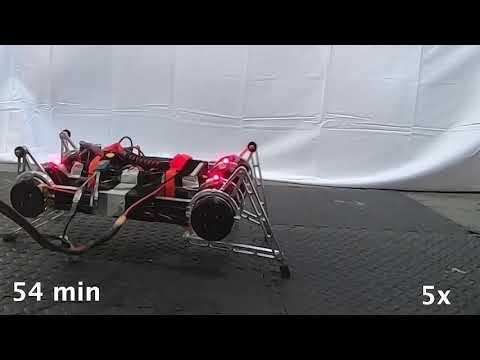
\includegraphics[width=\linewidth,height=0.4\textheight,keepaspectratio]{images/soft-actor-critic/figures/real-robot-1.jpg}\\[0.4em]
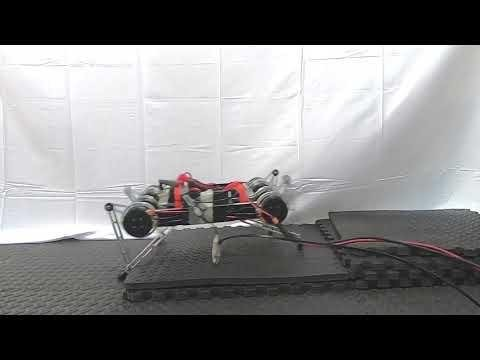
\includegraphics[width=\linewidth,height=0.4\textheight,keepaspectratio]{images/soft-actor-critic/figures/real-robot-2.jpg}
\end{column}
\end{columns}
\begin{flushright}
    \tiny\url{https://arxiv.org/abs/1812.05905}
\end{flushright}
\end{frame}
\begin{frame}{Real World Robots}
\begin{itemize}
    \item \textbf{Task:} a multi-fingered hand opens a valve to a target angle, learning from raw joint sensors \rref{2}
    \item End-to-end real-world learning in $\approx$20 hours wall-clock
    \item With valve angle exposed as input: \textbf{SAC 3 hours vs.\ PPO 7.4 hours} --- the off-policy, entropy-regularised advantage shows clearly in sample efficiency
\end{itemize}
\begin{figure}
    \centering
    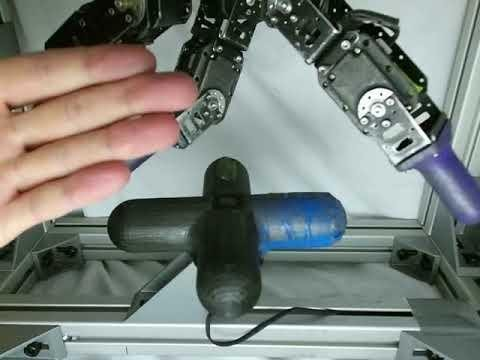
\includegraphics[width=0.55\textwidth,height=0.5\textheight,keepaspectratio]{images/soft-actor-critic/figures/dexterous-hand.jpg}
\end{figure}
\begin{flushright}
    \tiny\url{https://sites.google.com/view/sac-and-applications}
\end{flushright}
\end{frame}
